\documentclass[12pt]{article}
\usepackage[utf8]{inputenc}
\usepackage{listings}
\usepackage{xcolor}
\usepackage{geometry}
\geometry{a4paper, margin=1in}
\usepackage{hyperref}
\usepackage{graphicx}
\usepackage{array}
\usepackage{float}
\usepackage{amsmath}

\graphicspath{ {media/} }


\definecolor{centrale_red}{RGB}{178,33,51}

\geometry{a4paper, margin=1in}
\hypersetup{
    colorlinks=true,
    linkcolor=blue,
    filecolor=magenta,  
    urlcolor=cyan,
    pdftitle={Practice Session Report},
    pdfpagemode=FullScreen,
}

\lstset{
    language=Java,
    basicstyle=\ttfamily\footnotesize,
    keywordstyle=\color{blue}\bfseries,
    stringstyle=\color{red},
    commentstyle=\color{green},
    breaklines=true,
    frame=single,
    rulecolor=\color{gray},
    showspaces=false,
    showstringspaces=false,
}

\renewcommand{\contentsname}{Table of Contents}
\newcommand{\university}{\textit{\textbf{EST Safi}}}

\begin{document}

\begin{titlepage}
    \thispagestyle{empty}

        \vspace*{2cm}
        \Huge\textbf{\textcolor{centrale_red}{Java: Practice Session Report}} \\
        \vspace{1cm}

        \begin{minipage}{0.4\textwidth}
                \begin{flushleft} \large
                    \emph{\textbf{Prepared by:}}\\ 
                    Karim ELKHANOUFI
                \end{flushleft}
            \end{minipage}
            ~
            \begin{minipage}{0.4\textwidth}
                \begin{flushright} \large
					\emph{\textbf{Supervised by:}}\\
                    Leila ELKHROF
                \end{flushright}
            \end{minipage}

        \vfill
        \large{\today}
\end{titlepage}

\newpage

\tableofcontents

\newpage

\section{Introduction}
This practical work continues a project on employee management. After detailing earlier phases on employee and leave management, this document focuses on developing a Java application for managing employee entry and exit.

The project employs the MVC (Model-View-Controller) architecture, which separates data, business logic, and the user interface. It reinforces object-oriented programming (OOP) fundamentals while introducing GUI development with the Swing library, ensuring a clear, modular, and scalable code structure.

The application provides an efficient solution for managing employee data through an intuitive interface. It supports data import/export from external files, enabling easier manipulation and sharing. The MVC design ensures organized code, simplifying maintenance and feature expansion.

Key features include:
\begin{itemize}
  \item Managing (Add/Delete/Update) Employees and their Holidays.
  \item Importing employee data from external files.
  \item Exporting data for backup or sharing.
  \item Streamlined management of employee entries and exits through a user-friendly interface.
\end{itemize}
This report demonstrates the effective use of OOP and MVC principles while addressing the project’s input/output requirements.

\pagebreak

\section{Code Implementation}

\subsection{Main Class}

The class Main is responsible for creating the the Views
and initializing their Controllers.

\begin{lstlisting}
import Controller.*;
import Model.*;
import View.*;

public class Main {
  public static void main(String[] args) {
    JFrame frame = new JFrame();
    frame.setTitle("Employees & Holidays Management");
    frame.setDefaultCloseOperation(JFrame.EXIT_ON_CLOSE);
    frame.setSize(800, 500);

    // Employee
    JPanel eview = new EmployeeView();
    EmployeeModel em = new EmployeeModel();
    EmployeeController ec = new EmployeeController(em, (EmployeeView) eview);

    // Holiday
    JPanel hview = new HolidayView();
    HolidayModel hm = new HolidayModel();
    HolidayController hc = new HolidayController(hm, (HolidayView) hview);

    JTabbedPane tabbedPane = new JTabbedPane();
    frame.add(tabbedPane);
    tabbedPane.addTab("Employees", eview);
    tabbedPane.addTab("Holidays", hview);

    frame.setVisible(true);
  }
}
\end{lstlisting}

\pagebreak

\subsection{DAO}

The DAO package contains all the necessary classes and interfaces
for database connectivity.

Employee and Holiday DAO both implement the Generic DAO interface
and uses DBConnection for database connection.

\subsubsection{DBConnection Class}
\begin{lstlisting}
package DAO;

public class DBConnection {
  private String url = "jdbc:postgresql://localhost:5432/java_db";
  private String dbuser = "postgres";
  private String dbpw = "pg1234";

  private static Connection con = null;

  public DBConnection() {
    if (con != null) return;
    try {
      Class.forName("org.postgresql.Driver");
      con = DriverManager.getConnection(url, dbuser, dbpw);
      System.out.println("DataBase Connection established!!");
    } catch (Exception e) {
      System.err.println(e);
    }
  }

  public Connection getConnection() {
    return con;
  }
}
\end{lstlisting}

\subsubsection{DAO Genetic Interface}
\begin{lstlisting}
package DAO;

import java.util.List;

public interface GenericDAOI<T> {
  public List<T> getAll();
  public T findById(int id);
  public boolean add(T m);
  public boolean delete(int id);
  public boolean update(int id, T m);
}
\end{lstlisting}

\pagebreak

\subsubsection{Data Import/Export Interface}
\begin{lstlisting}
package DAO;

import java.io.IOException;
import java.util.List;

public interface DataImportExport<T> {
  void importData(String filename) throws IOException;
  void exportData(String filename, List<T> data) throws IOException;
}
\end{lstlisting}


\subsubsection{Employee DAO Implementation}
\begin{lstlisting}
package DAO;

import Model.EmployeeModel;

public class EmployeeDAOImpl
    implements GenericDAOI<EmployeeModel>, DataImportExport<EmployeeModel> {
  private Connection con = null;

  public EmployeeDAOImpl() {
    con = new DBConnection().getConnection();
  }

  @Override
  public boolean add(EmployeeModel m) { // implementation }

  @Override
  public boolean delete(int id) {}

  @Override
  public boolean update(int id, EmployeeModel m) {}

  @Override
  public ArrayList<EmployeeModel> getAll() {}

  @Override
  public EmployeeModel findById(int id) {}

  @Override
  public void importData(String filename) throws IOException;

  @Override
  public void exportData(String filename, List<EmployeeModel> data) throws IOException;
}
\end{lstlisting}

\pagebreak

\subsubsection{Holiday DAO Implementation}
\begin{lstlisting}
package DAO;

import Model.HolidayModel;

public class HolidayDAOImpl implements GenericDAOI<HolidayModel>, DataImportExport<HolidayModel> {
  private Connection con = null;

  public HolidayDAOImpl() {
    con = new DBConnection().getConnection();
  }

  @Override
  public List<HolidayModel> getAll() { // implementation }

  @Override
  public HolidayModel findById(int id) {}

  @Override
  public boolean add(HolidayModel h) {}

  @Override
  public boolean delete(int id) {}

  @Override
  public boolean update(int id, HolidayModel h) {}

  public int updateSolde(int id, int decriment) {}

  @Override
  public void exportData(String filename, List<HolidayModel> data) throws IOException;

  @Override
   public void importData(String filename) throws IOException; // Not Used
}

\end{lstlisting}

\pagebreak

\subsection{Models}

The Model package contains the necessary classes that interfaces
between the Controllers and The DAO layers.

\subsubsection{Employee Model}
\begin{lstlisting}
package Model;

import DAO.EmployeeDAOImpl;

public class EmployeeModel {
  private EmployeeDAOImpl dao = null;
  private String lname, fname, email, phone, post, role;
  private double salary;
  private int id, solde;

  public enum Post {
    STUDY_AND_DEV_ENGINEER,
    TEAM_LEADER,
    PILOTE
  };

  public enum Role {
    ADMIN,
    EMPLOYEE
  };

  public EmployeeModel(String lname, String fname, String email,
  String phone, double salary, String post, String role);

  // Getters
  public int getId();
  // ...

  // Setters
  public void setId(int id);
  // ...

  public boolean addEmployee()
  public boolean deleteEmployee(int id);
  public boolean updateEmployee(int id);
  public ArrayList<EmployeeModel> getAllEmployees();

  public void importData(String filepath) throws IOException;
  public void exportData(String filepath, List<EmployeeModel> data) throws IOException;
  private boolean checkIfFileExists(File file) throws IllegalArgumentException;
  private boolean checksIsFile(File file) throws IllegalArgumentException;
  private boolean checksIsReadable(File file) throws IllegalArgumentException;

  @Override
  public String toString();
}
\end{lstlisting}

\pagebreak

\subsubsection{Holiday Model}
\begin{lstlisting}
package Model;

import DAO.HolidayDAOImpl;

public class HolidayModel {
  private HolidayDAOImpl dao = null;

  private int eid, id;
  private String EmployeeName;
  private String startDate;
  private String endDate;
  private String type;

  private DateTimeFormatter formatter = DateTimeFormatter.ofPattern("yyyy-MM-dd");

  public enum HolidayType {
    Payed_holiday,
    Unpayed_holiday,
    Sickness_holiday
  };

  // Constructors
  public HolidayModel();
  public HolidayModel(HolidayDAOImpl dao);
  public HolidayModel(int eid, String startDate, String endDate, String type);
  public HolidayModel(ResultSet rs);

  // Getters
  public int getId();
  // ...

  // Setters
  public void setId(int id);
  // ...

  // Methods
  public boolean addHoliday();
  public boolean deleteHoliday(int id);
  public boolean updateHoliday(int id, HolidayModel n);
  public List<HolidayModel> getAllHolidys();
  public HolidayModel findHolidayById(int id);

  public void importData(String filepath) throws IOException;
  public void exportData(String filepath, List<EmployeeModel> data) throws IOException;
  private boolean checkIfFileExists(File file) throws IllegalArgumentException;
  private boolean checksIsFile(File file) throws IllegalArgumentException;
  private boolean checksIsReadable(File file) throws IllegalArgumentException;

  @Override
  public String toString();
\end{lstlisting}

\pagebreak

\subsection{Controllers}

The Controller package includes the necessary Classes for controlling
and managing the View and its events.

\subsubsection{Employee Controller}
\begin{lstlisting}
package Controller;

import Model.EmployeeModel;
import View.EmployeeView;

public class EmployeeController {

  private EmployeeView view;
  private EmployeeModel model;
  private int selectedRow = -1;

  public EmployeeController(EmployeeModel model, EmployeeView view) {
    this.model = model;
    this.view = view;
    populateTable();
    initAddEvent();
    initDeleteEvent();
    initUpdateEvent();
    initShowEvent();
    initFillEvent();
    initTableEvents();
    initImportBtn();
    initExportBtn();
  }

  private void initAddEvent();
  private void initDeleteEvent();
  private void initUpdateEvent();
  private void initShowEvent();
  private void initFillEvent();
  private void initTableEvents();
  private void initImportBtn();
  private void initExportBtn();

  public void populateTable();
  public void fillFields();
  public void emptyFields();

  private void handleImport();
  private void handleExport();
}
\end{lstlisting}

\pagebreak

\subsubsection{Holiday Controller}
NOTE: Can I use another model in my controller
\begin{lstlisting}
package Controller;

import Model.EmployeeModel;
import Model.HolidayModel;
import View.HolidayView;

public class HolidayController {
  private HolidayModel model = null;
  private HolidayView view = null;
  private int selectedRow = -1;

  public HolidayController(HolidayModel model, HolidayView view) {
    this.model = model;
    this.view = view;
    initTableEvent();
    populateFields();
    populateTable();
    initAddEvent();
    initDeleteEvent();
    initUpdateEvent();
    initRefreshEvent();
    initExportBtn();
  }

  public void initAddEvent();
  public void initDeleteEvent();
  public void initUpdateEvent();
  public void initRefreshEvent();
  public void initTableEvent();
  public void populateTable();
  public void populateFields();
  public void emptyFields();

  private void initExportBtn();
  private void handleExport();
}
\end{lstlisting}

\pagebreak

\subsection{Views}

The View package that holds all the GUI representations that gonna be
managed by the controllers.

\subsubsection{Employee View}
\begin{lstlisting}
package View;

import Model.EmployeeModel.Post;
import Model.EmployeeModel.Role;

public class EmployeeView extends JPanel {

  public JButton addBtn = new JButton("Add");
  public JButton deleteBtn = new JButton("Delete");
  public JButton updateBtn = new JButton("Update");
  public JButton showBtn = new JButton("Show");
  public JButton fillBtn = new JButton("Fill");
  public JButton importBtn = new JButton("Import");
  public JButton exportBtn = new JButton("Export");

  public JTextField lnameField = new JTextField();
  public JTextField fnameField = new JTextField();
  public JTextField emailField = new JTextField();
  public JTextField phoneField = new JTextField();
  public JTextField salaryField = new JTextField();

  public JComboBox<Role> roleComboBox = new JComboBox<>(Role.values());
  public JComboBox<Post> postComboBox = new JComboBox<>(Post.values());

  public JTable table = new JTable();

  public EmployeeView();
  public void showSuccess(String message);
  public void showFailure(String message);
}
\end{lstlisting}

\pagebreak

\subsubsection{Holiday View}
\begin{lstlisting}
package View;

import Model.HolidayModel.HolidayType;

public class HolidayView extends JPanel {
  public JButton addBtn = new JButton("Add");
  public JButton deleteBtn = new JButton("Delete");
  public JButton updateBtn = new JButton("Update");
  public JButton refreshBtn = new JButton("Refresh");
  public JButton exportBtn = new JButton("Export");

  public JComboBox<String> employeeField = new JComboBox<>();
  public JComboBox<HolidayType> typeField = new JComboBox<>(HolidayType.values());
  public JTextField startDateField = new JTextField();
  public JTextField endDateField = new JTextField();

  public JTable table = new JTable();

  public HolidayView();
  public int getEid();
  public String getType();
  public String getStartDate();
  public String getEndDate();
  public void showSuccess(String message);
  public void showFailure(String message);
}
\end{lstlisting}

\pagebreak

\section{Demonstration}

The application was tested on Ubuntu with PostgreSQL as the
database management system, Compiled and Ran using openjdk 17.

\vspace{0.6cm}

The following figure represents the Employee tab that enables
the user to perform various actions, such as adding, deleting,
updating, and viewing employee records.

\begin{figure}[H]
  \centering
  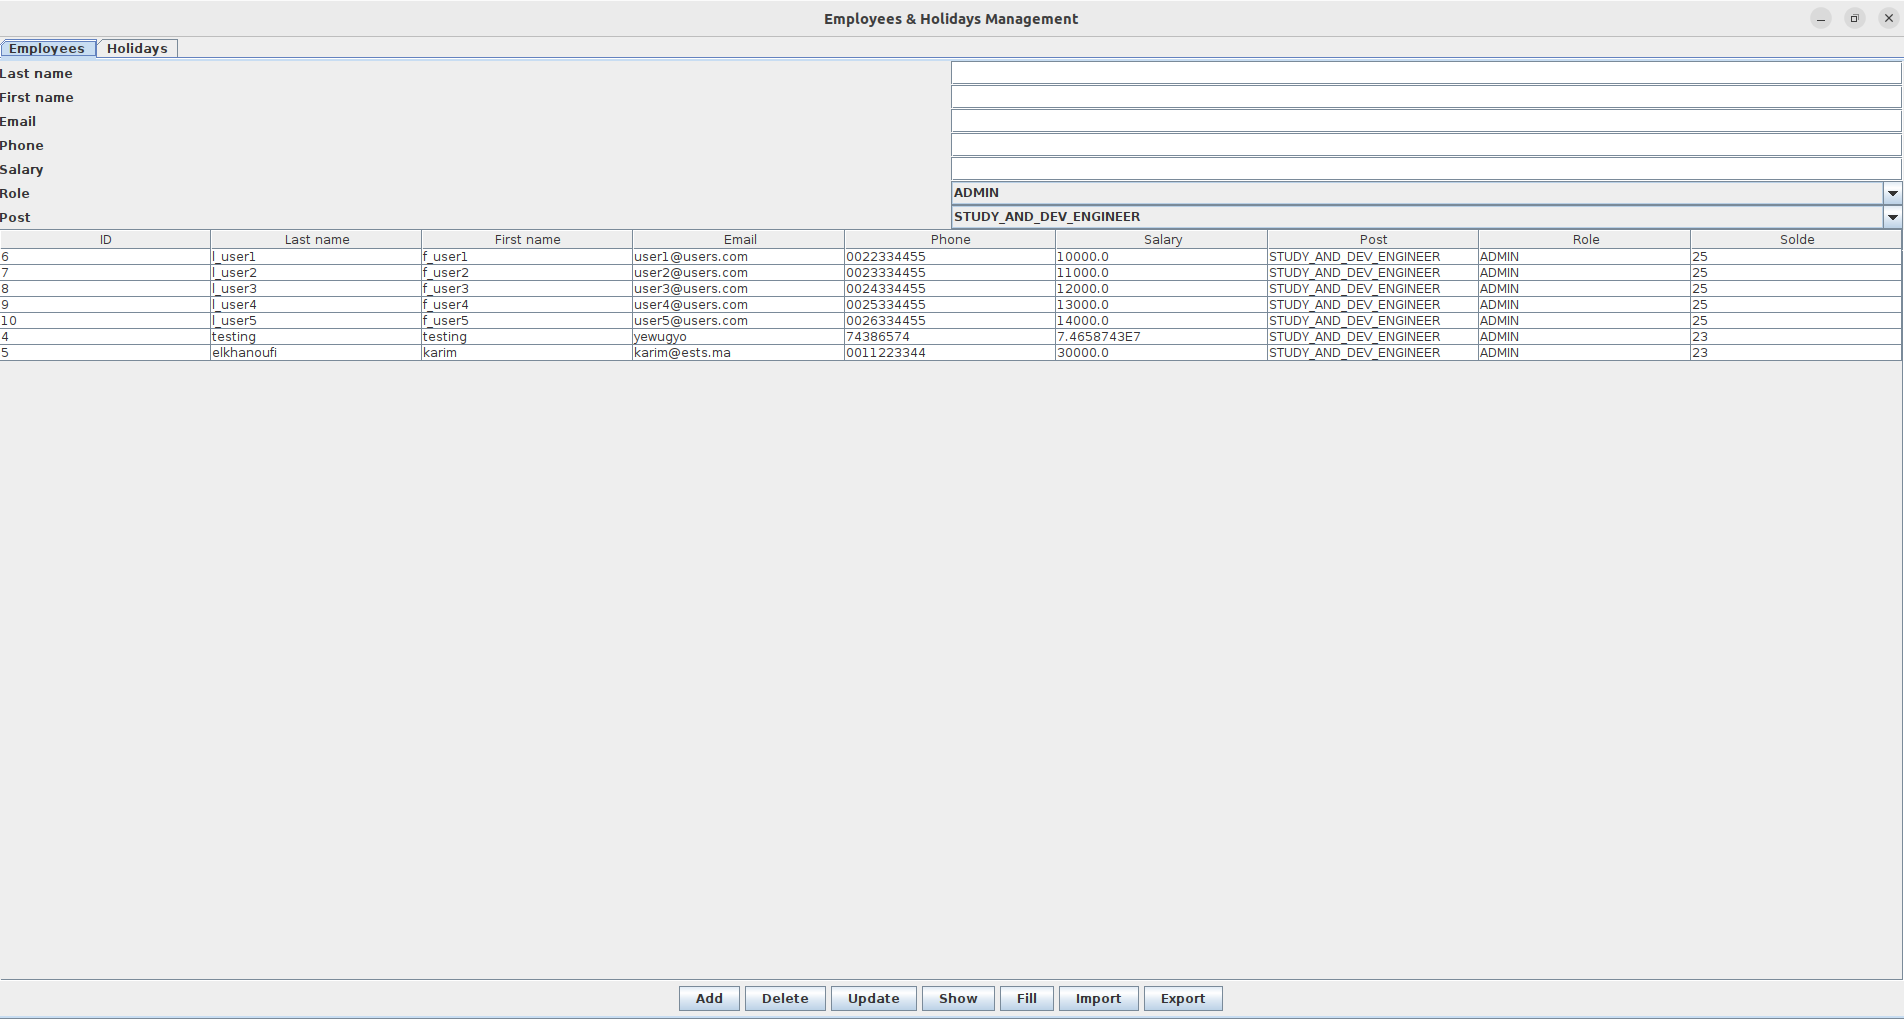
\includegraphics[width=0.9\textwidth]{employee_preview.png}
  \caption{Screenshot of the Employee Management System GUI}
\end{figure}

Each button is responsible for an action:

\begin{itemize}
    \item \textbf{Add}* - add an employee
    \item \textbf{Delete}** - delete an employee
    \item \textbf{Update}*** - update an employee
    \item \textbf{Show} - show/refresh data
    \item \textbf{Fill}* - fill inputs from the selected table record
    \item \textbf{Import} - import data (Employees) from an CSV file
    \item  \textbf{Export} - export data in CSV format 
\end{itemize}

\noindent \text{*} - inputs should be full\\
\text{**} - a table record should be selected\\
\text{***} - both the above

\pagebreak

And the following figure represents the Holiday view that enable
the user to add, update and delete the holidays assigned to the
employees.

\begin{figure}[H]
  \centering
  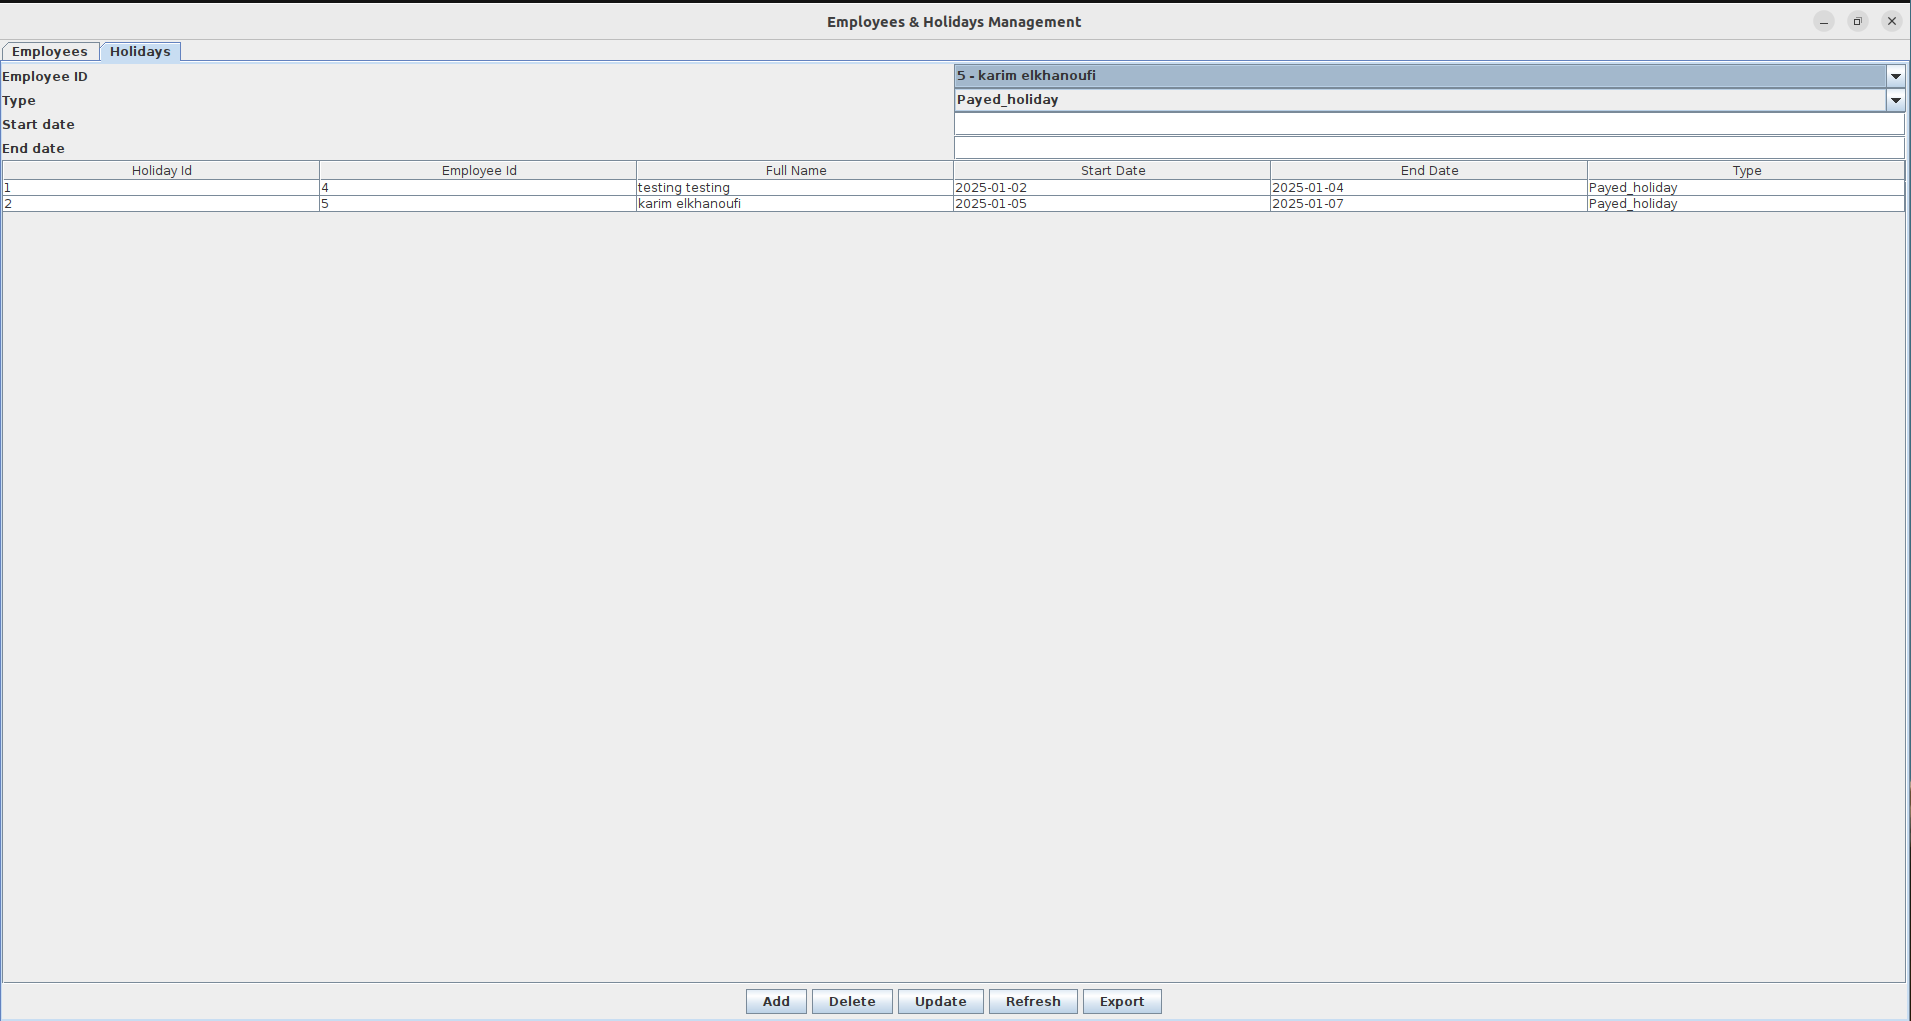
\includegraphics[width=0.9\textwidth]{holiday_preview.png}
  \caption{Screenshot of the Holiday Management System GUI}
\end{figure}

\begin{itemize}
    \item \textbf{Add}* - add an holiday
    \item \textbf{Delete}** - delete an holiday
	\item \textbf{Update}*** - update an holiday
    \item \textbf{Refresh} - refresh data
    \item  \textbf{Export} - export data (Employees with holidays) in CSV format
\end{itemize}

\noindent \text{*} - inputs should be full\\
\text{**} - a table record should be selected\\
\text{***} - both the above

\pagebreak

\section{References}
\begin{itemize}
    \item \href{https://docs.oracle.com/en/java/}{Java Documentation}
    \item \href{https://www.postgresql.org/docs/}{PostgreSQL Documentation}
    \item \href{https://jdbc.postgresql.org/documentation/}{pgJDBC Documentation}
\end{itemize}

\end{document}
